\begin{figure}[H]
  \centering
  % Primer grafo (G_1)
  \begin{minipage}[t]{0.49\textwidth}
    \centering
    \scalebox{0.7}{% Ajusta este valor (ej. 0.6, 0.7, 0.8) para controlar el tamaño
      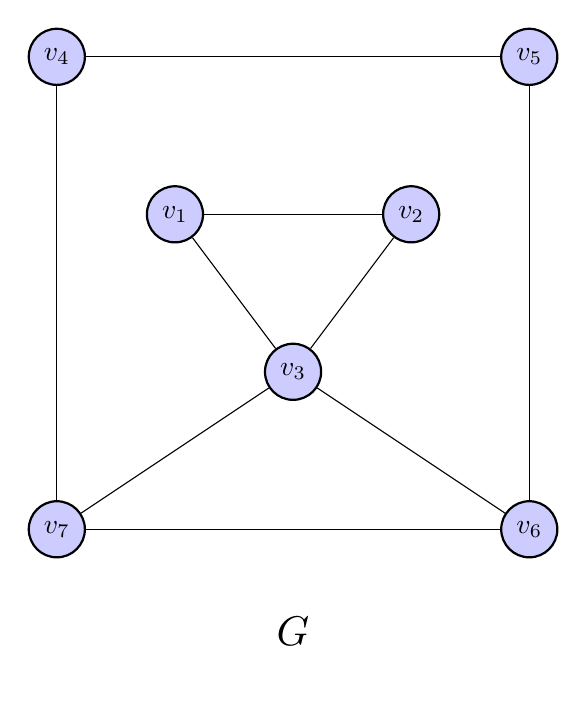
\begin{tikzpicture}[auto=left,every node/.style={circle,fill=blue!20,draw=black,thick}]
  % Cuadrado exterior (v4 y v5 en la parte superior; v7 y v6 en la parte inferior)
  \node (v4) at (-3, 3.5) {$v_4$};
  \node (v5) at (3, 3.5) {$v_5$};
  \node (v6) at (3, -2.5) {$v_6$};
  \node (v7) at (-3, -2.5) {$v_7$};

  % Triángulo interior (v1, v2, v3)
  \node (v1) at (-1.5, 1.5) {$v_1$};
  \node (v2) at (1.5, 1.5) {$v_2$};
  \node (v3) at (0, -0.5) {$v_3$};

  % Aristas del cuadrado exterior
  \foreach \from/\to in {v4/v5, v5/v6, v6/v7, v7/v4}
    \draw (\from) -- (\to);

  % Aristas del triángulo interior
  \foreach \from/\to in {v1/v2, v2/v3, v3/v1}
    \draw (\from) -- (\to);

  % Conexiones del vértice inferior v3 a las esquinas inferiores
  \draw (v3) -- (v7);
  \draw (v3) -- (v6);

  % Título
  \node[draw=none, fill=none, scale=1.5] at (0,-3.8) {$G$};
\end{tikzpicture}

    }
  \end{minipage}%
  \hspace{-3em}%
  % Segundo grafo (G'_1)
  \begin{minipage}[t]{0.49\textwidth}
    \centering
    \scalebox{0.7}{% Usa el mismo factor de escala para que guarden proporción
      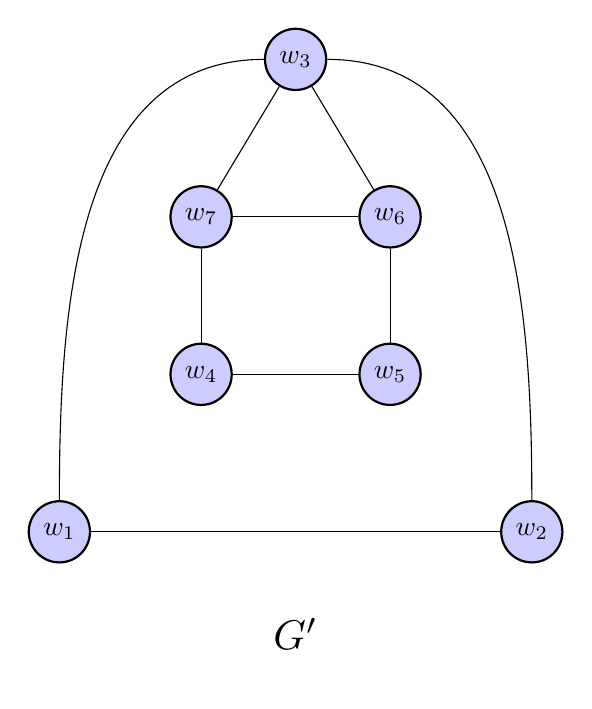
\begin{tikzpicture}[auto=left,every node/.style={circle,fill=blue!20,draw=black,thick}]
  % Vértice superior en la misma cota máxima (y=3.5)
  \node (w3) at (0, 3.5) {$w_3$};

  % "Casa" interior (w7, w6, w5, w4)
  \node (w7) at (-1.2, 1.5) {$w_7$};
  \node (w6) at (1.2, 1.5) {$w_6$};
  \node (w5) at (1.2, -0.5) {$w_5$};
  \node (w4) at (-1.2, -0.5) {$w_4$};

  % Vértices inferiores en la misma cota mínima (y=-2.5)
  \node (w1) at (-3, -2.5) {$w_1$};
  \node (w2) at (3, -2.5) {$w_2$};

  % Aristas de la estructura interior
  \foreach \from/\to in {w7/w6, w6/w5, w5/w4, w4/w7, w3/w7, w3/w6}
    \draw (\from) -- (\to);

  % Arista de la base exterior
  \draw (w1) -- (w2);

  % Arcos exteriores curvados
  \draw (w3) to[out=180, in=90] (w1);
  \draw (w3) to[out=0, in=90] (w2);

  % Título
  \node[draw=none, fill=none, scale=1.5] at (0,-3.8) {$G'$};
\end{tikzpicture}

    }
  \end{minipage}
  
  \caption{$G$ y $G'$ son isomorfos}
  \label{fig:primer_isomorfismo}
\end{figure}
